\subsection{Red de grafos generada por el RNA}

 La información exportada en el Código \ref{lst:EJ1_5}, Código \ref{lst:EJ1_6} y Código \ref{lst:EJ1_7} es utilizada resumida por el RNA para una mejor interpretacion. El resultado de este resumen se ilustra en el diagrama de la Figura \ref{fig:EJ1_8}.

	\begin{figure}[H]
		\centering
		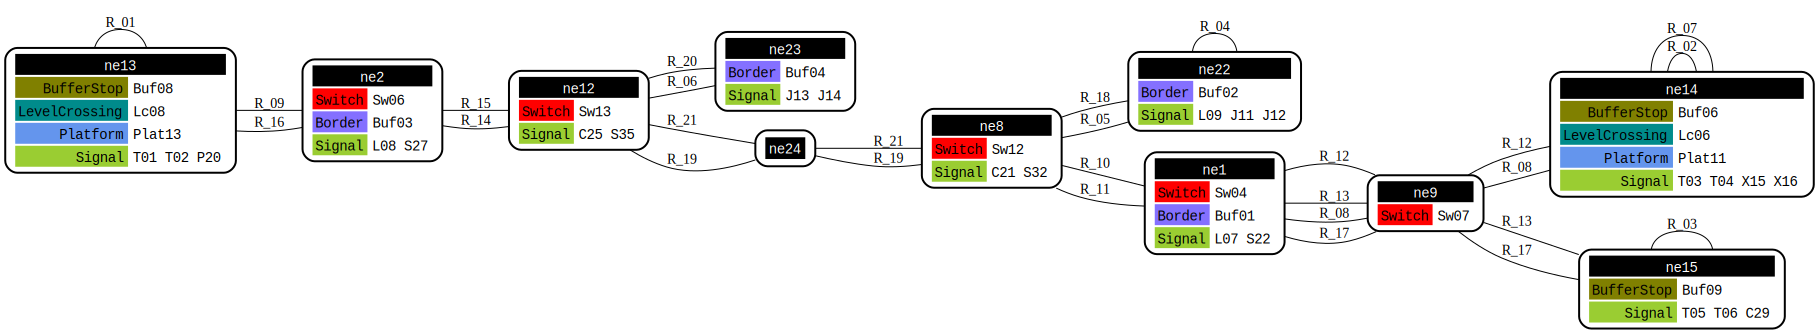
\includegraphics[angle = 90, origin = c, width=0.25\textwidth]{Figuras/Graph_1}
		\centering\caption{Red de grafos generada por el RNA para el ejemplo 1.}
		\label{fig:EJ1_8}
	\end{figure}
	
	Cada nodo del grafo de la Figura \ref{fig:EJ1_8} corresponde a un \textit{netElement}. En cada nodo se listan todos los elementos ferroviarios contenidos por en \textit{netElement}. Las aristas del grafo son las rutas que los conectan. De esta manera, es posible detectar visualmente cualquier nodo aislado de la red o nodos que solo son accedidos en un sentido. Por ejemplo, si algún entre dos nodos no existe una cantidad par de rutas, entonces solamente se puede circular entre esos nodos en un solo sentido.